\section{Theory}\label{sec:pid_theory}

In closed loop systems, there is always a process variable which works as a system parameter that needs to be controlled. The output of these systems is measured using a sensor and its value is compared with a setpoint (reference). A feedback allows a constant monitorization of the process because the error between the reference and the process variable is used as a controller input. Then, the controller executes some calculations that will act in the plant. The type of control chosen for this project was the PID control, where the controller can be proportional, derivative, integral or a combination between them. %Introduce these controllers because there are more than these ones. What is a goal of a controller. what do you use it for

The proportional controller has its output always proportional to the error (input of the controller). This type of controller is responsible for reducing the rise time and the steady state error (SSE). Decreasing the rise time results from the increase of the proportional gain, and the steady state error corresponds to the difference between the output and the desired value. The previous difference is proportional to the output of the controller which will also be the input of the plant. The proportional gain, $K_P$, is inversely proportional to the SSE but, after a certain value of reduction on this error, increasing the value of $K_P$ only leads to overshoot of the system response. On the contrary, reducing $K_P$ will not allow the elimination of the steady state error of the system. 

\begin{figure}[H]
	\centering
	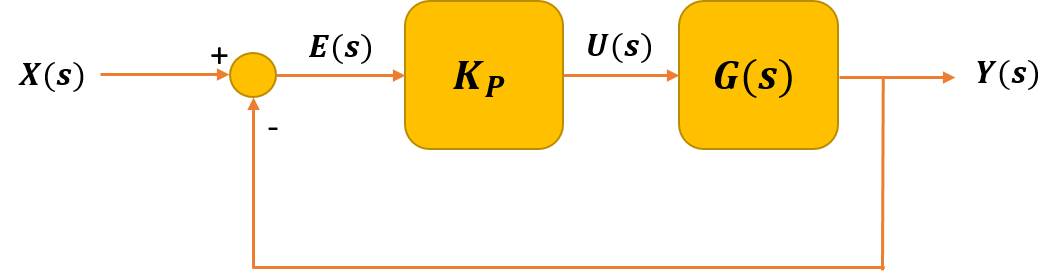
\includegraphics[scale=0.6]{figures/propor_controller.png}
	\caption{System controller by a proportional term}
	\label{propor_controller}
\end{figure}

Based on the system of the figure \ref{propor_controller} and considering the plant $G(s)$ described in the equation \ref{system_equation} it is possible to calculate the characteristic equation (equations \ref{charac_equation1} and \ref{charac_prop_system}). The linear plant $G(s)$ is a second order plant that represents a good balance between the real-life and the amount of required calculations.

\begin{equation}\label{system_equation}
G(s)= \frac{A}{s^2 + a_{1}s + a_{2}}
\end{equation}

\begin{equation}\label{charac_equation1}
1 + K_PG(s)=0
\end{equation}

\begin{equation}\label{charac_prop_system}
s^2 + a_{1}s + a_{2} + K_PA=0
\end{equation}

The equation \ref{charac_prop_system} shows the possibility of controlling the constant term $(a_{2} + K_PA)$ which determines the natural frequency but cannot control the damping term $a_{1}$ since it is independent of $K_{P}$. Therefore, the overshoot of the system response is a consequence of the lack of control of the damping term.

In addition, these controllers provide a smaller amplitude and phase margin (the overshoot described before happens when the phase margin is too small), a faster dynamics satisfying wider frequency band and larger sensitivity to the noise (because of the proportionality between the error and the output of the controller).

\vspace{5mm}

The integral component, described in figure \ref{integ_controller}, sums the error term over time which means that even a small error will increase slowly the integral component. This behaviour tends the steady state error to zero because the integral response will continually increase over time unless the error is zero. However, since the integral term responds to accumulated errors from the past, it can cause the present value to overshoot the setpoint value.

\begin{figure}[H]
	\centering
	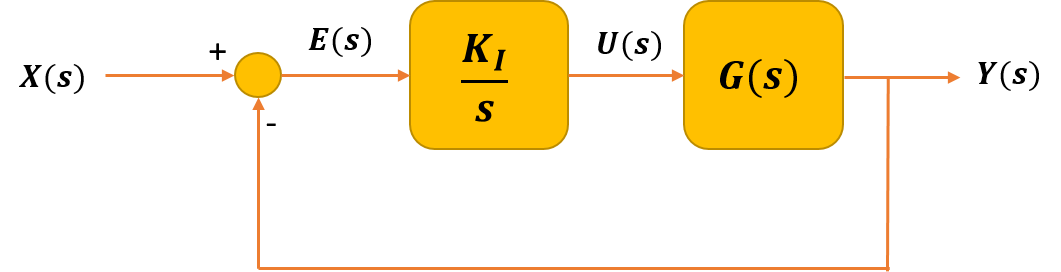
\includegraphics[scale=0.6]{figures/integ_controller.png}
	\caption{System with a integral controller}
	\label{integ_controller}
\end{figure}

Considering the same plant (equation \ref{system_equation}) it is possible to verify that the closed-loop transfer function is given by the equation \ref{int_TF} and the relation between the input and the error is defined in the equation \ref{int_error_input}.

\begin{equation}\label{int_TF}
\frac{Y(s)}{X(s)}= \frac{K_IG(s)}{s + K_IG(s)}
\end{equation}

\begin{equation}\label{int_error_input}
\frac{E(s)}{X(s)}= \frac{s}{s + K_IG(s)}
\end{equation}

Using the Final Value Theorem, it is possible to calculate the error in the infinite that should be zero (the steady state error will be zero). In the equation \ref{limit_sse}, the steady state error of the system for a step input ($X(s)=\frac{1}{s}$) is calculated . The result is independent of the input, which mean that, in the infinite, the error will be always zero.

\begin{equation}\label{limit_sse}
\lim_{t\to\infty} e(t) = \lim_{s \to 0} sE(s) = \lim_{s \to 0} s\frac{s}{s + K_IG(s)}\frac{1}{s} = 0
\end{equation}

\vspace{5mm}

The derivative feedback, also called rate feedback, is proportional to the rate of change of the system's error, which means that the slope of the error function over time is calculated. Knowing the trend of the error signal, these calculations allow to have an anticipatory behaviour. Thus, the stability of the closed-loop system is improved as well as the speed of the transient response and the overshoot. Derivative acts as a brake on the control effort because the more the controller tries to change the value, the more it counteracts the effort, unabling violent changes. The derivative response is also highly sensitive to noise which means that the control system can be unstable if the sensor feedback is noisy. 

\begin{figure}[H]
	\centering
	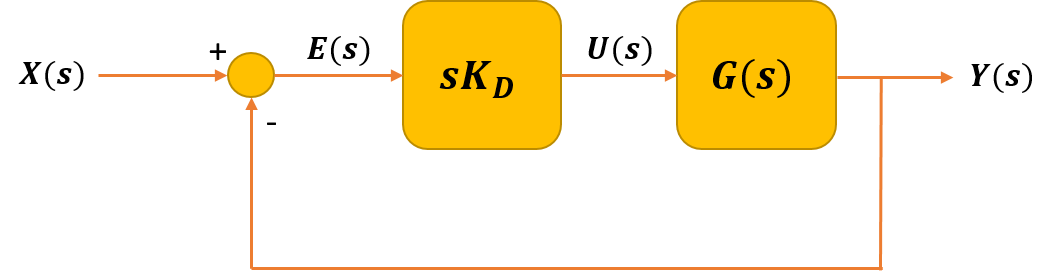
\includegraphics[scale=0.6]{figures/deriv_controller.png}
	\caption{System with a derivative controller}
	\label{deriv_controller}
\end{figure}

Based on the system of the figure \ref{deriv_controller} it is possible to build the relation between the input of the plant and the error between the desired and the output values. This relation is described in the equation \ref{deri_relation}.

\begin{equation}\label{deri_relation}
\frac{U(s)}{E(s)}= sK_D
\end{equation}

\vspace{5mm}

The PI controller (figure \ref{PI_controller}) is constituted by a proportional and an integral part and it is mainly used to eliminate the steady state error resulting from the proportional component. However, this controller has a negative impact in the speed of the response (compared to the proportional controller) and in the stability of the system. Hence, this controller should be applied when speed is not an important parameter. %Due to the fact that PI response does not predict the future errors of the system, the rise time can not be decreased and the oscillations can not be eliminated.

\begin{figure}[H]
	\centering
	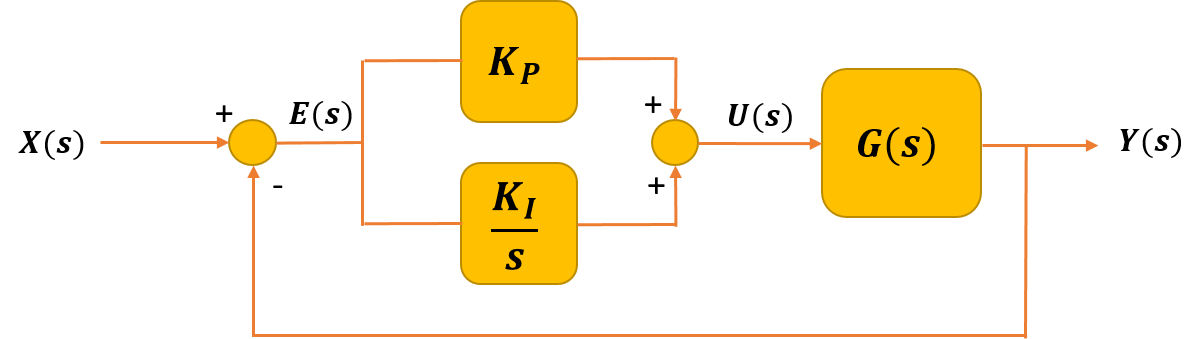
\includegraphics[scale=0.6]{figures/PI_controller.png}
	\caption{System with a PI controller}
	\label{PI_controller}
\end{figure}

Hence, the equation \ref{PI_equation} describes the behaviour of the PI controller.

\begin{equation}\label{PI_equation}
\frac{U(s)}{E(s)}= K_P + \frac{K_I}{s}
\end{equation}

\vspace{5mm}

The derivative control is almost never used by itself because it does not supply information on the desired end state. Hence, a proporcional term is needed in order to achive the desired end state, resulting in a PD controller (figure \ref{PD_controller}). In addition, if $e(t)$ remains constant, the output of a derivative part controller would be zero and a proportional component would be needed to provide a control signal at this time. The PD controllers are, thus, more stable than the proportional ones but they are also slower than the same ones because the derivative part prevents the sudden changes occuring.

\begin{figure}[H]
	\centering
	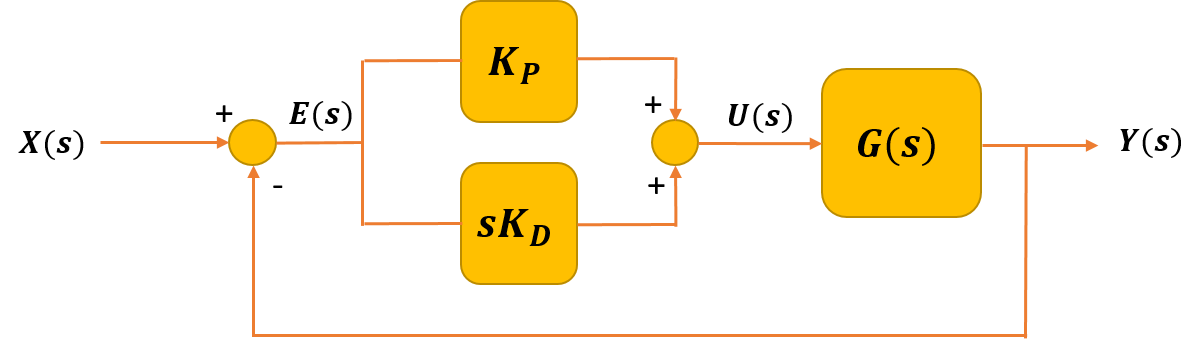
\includegraphics[scale=0.6]{figures/PD_controller.png}
	\caption{System with a PD controller}
	\label{PD_controller}
\end{figure}

\vspace{5mm}

The PID controller collects the proportional, integral and derivative parts which allows to have a zero steady state error, a fast response and a higher stability. The derivative component that is added to the PI controller allows the reduction of the overshoot and the oscillations that occur in the output response of the system. 

\begin{figure}[H]
	\centering
	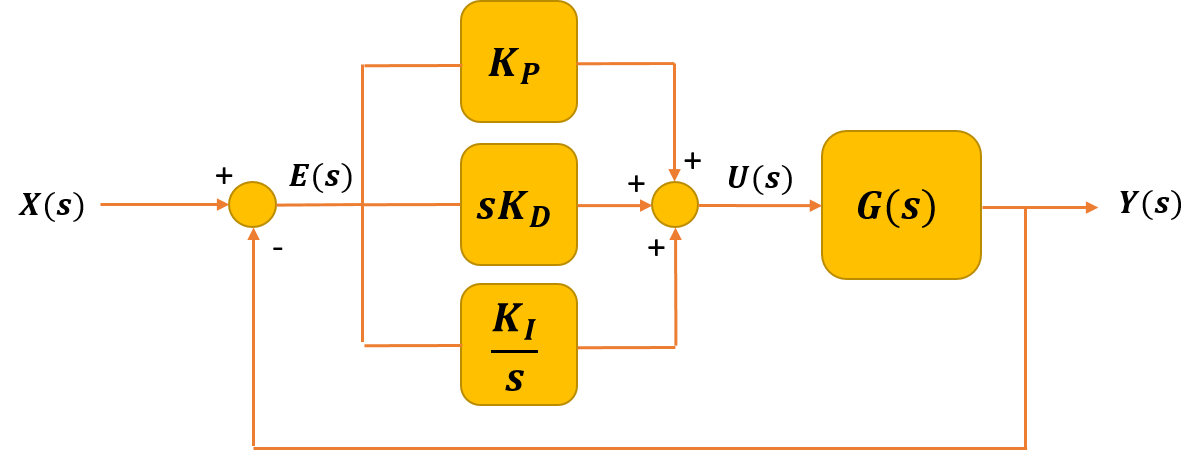
\includegraphics[scale=0.6]{figures/PID_controller.png}
	\caption{System with a PID controller}
	\label{PID_controller}
\end{figure}

In this project P, PI, PD and PID controllers were tested and for every case the behaviour was analysed. These analyses are presented in the next section.